
\documentclass{article}

\usepackage{fullpage}
\usepackage{graphicx}
\usepackage{amsmath}
\usepackage{textcomp}

\title{Incompressible Energy Equation Simulation}
\author{Michael Deakin}

\begin{document}
\maketitle

\begin{section}{Introduction}

In this report, I describe the properties of the implicit euler solver written for the energy equation.
I also compare it to the RK4 and RK1 solvers.
Unfortunately, due to time constraints, I was unable to find the cause of instability in my solvers, so the report is incomplete at this point in time.
\end{section}

\begin{section}{Spatial Discretization}
The solvers implemented a second order centered finite volume discretization to approximate the temperature.
These were tested with the equations described in part 1 to verify second order accuracy;
the results can be generated by running the 'energy\_tester' application. In this, the average order of accuracy over a series of meshes is found to be $\sim 2.0$ for the x, y, dx, and dy fluxes.
For a $40 \times 40$ mesh, these had L1 errors of $0.5$, $0.5$, $2.1$, and $0.52$, respectively.
For a $80 \times 80$ mesh, these had L1 errors of $0.5$, $0.5$, $2.1$, and $0.52$, respectively.
For a $160 \times 160$ mesh, these had L1 errors of $0.5$, $0.5$, $2.1$, and $0.52$, respectively.
For a $320 \times 320$ mesh, these had L1 errors of $0.5$, $0.5$, $2.1$, and $0.52$, respectively.
That these are not decreasing with increasing mesh size suggests the error is concentrated in some terms which are only first order accurate; likely the boundaries.
Combining these into the flux integral is also found to have an average accuracy order of convergence of $2$, as expected.
The source term was implemented as a finite difference discretization,
it was also found to have 2nd order convergence, with L1 errors of $0.05$.

Figures of the errors in the spatial discretization calculations are shown in Figure \ref{space_errs}.
All of these look reasonable, though the error at the boundaries of the $\frac{dT}{dx}$ flux is somewhat concerning,
as the other errors are in the range of $\text{e}-5$, rather than $\text{e}-2$.
The code appears correct, though, so it's not clear what the cause is.

\begin{figure}[h]
  \centering{
    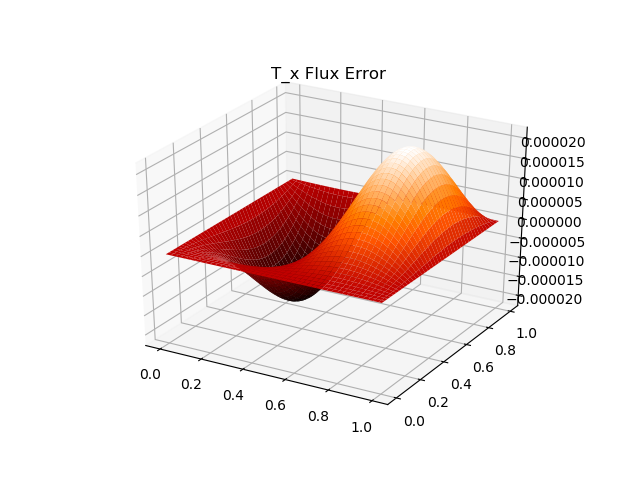
\includegraphics[width=0.45\textwidth]{figs/x_flux_err.png}
    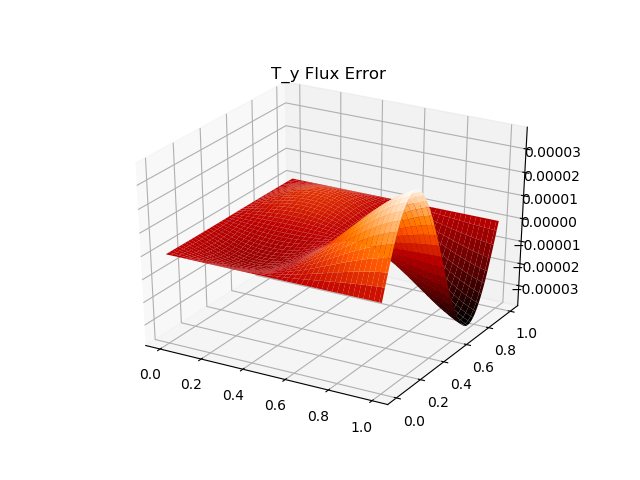
\includegraphics[width=0.45\textwidth]{figs/y_flux_err.png}
    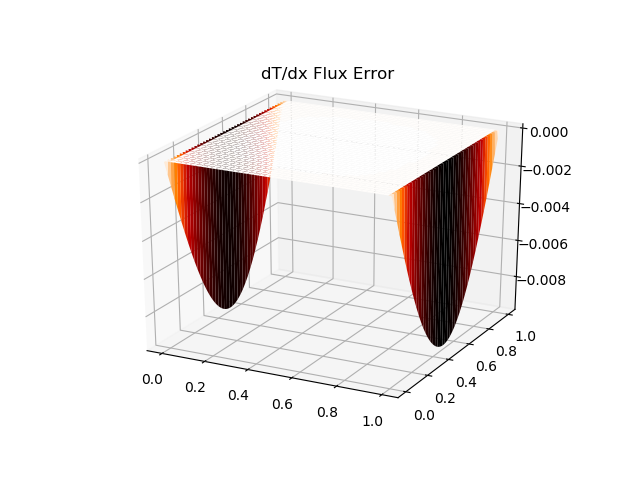
\includegraphics[width=0.45\textwidth]{figs/dt_dx_flux_err.png}
    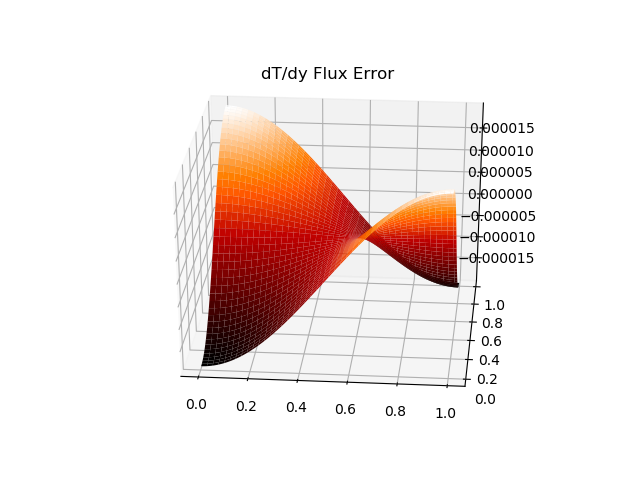
\includegraphics[width=0.45\textwidth]{figs/dt_dy_flux_err.png}
    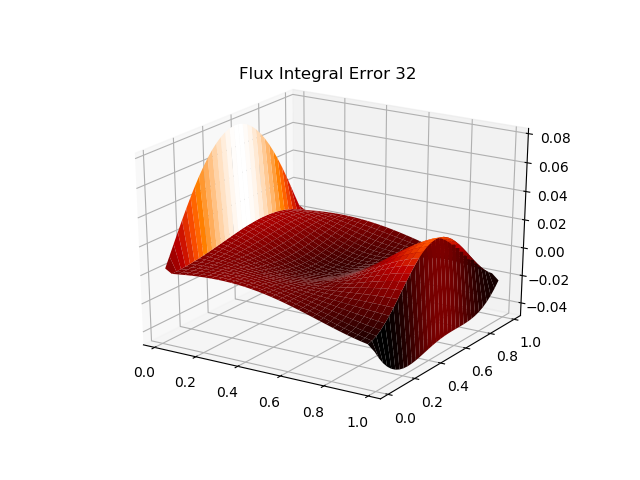
\includegraphics[width=0.45\textwidth]{figs/flux_int_32_err.png}
    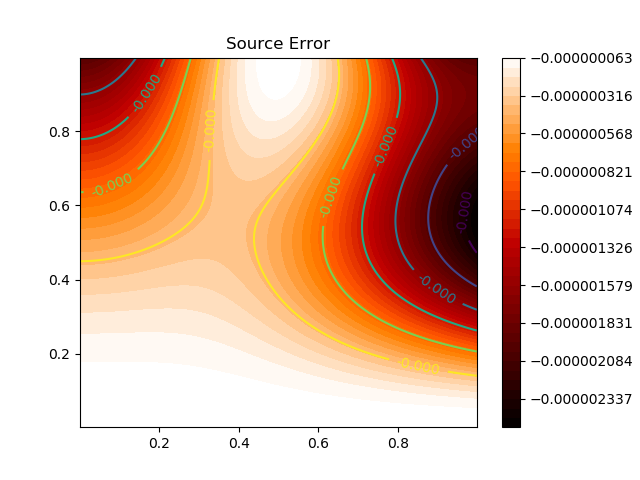
\includegraphics[width=0.45\textwidth]{figs/source_err.png}
  }
  \label{space_errs}
  \caption{{\bf From left to right, top to bottom:} Errors in the $T_x$, $T_y$,
    $\frac{dT}{dx}$ and $\frac{dT}{dy}$ fluxes, the flux integral, and the source term}
\end{figure}
\end{section}

\begin{section}{Time Discretization}
Three time discretizations were implemented: RK1, RK4, and Implicit Euler.
The boundary conditions for the implicit solver are not implemented correctly yet.
As a result, it's clearly not (currently!) second order accurate.
The explicit solver seems to be stable for the boundary conditions
(assuming they're implemented correctly) imposed by question 5 and 7,
figures of the fully developed profile are in Figures \ref{exp_part5} and \ref{exp_part7}.

\begin{figure}[ht]
  \centering{
    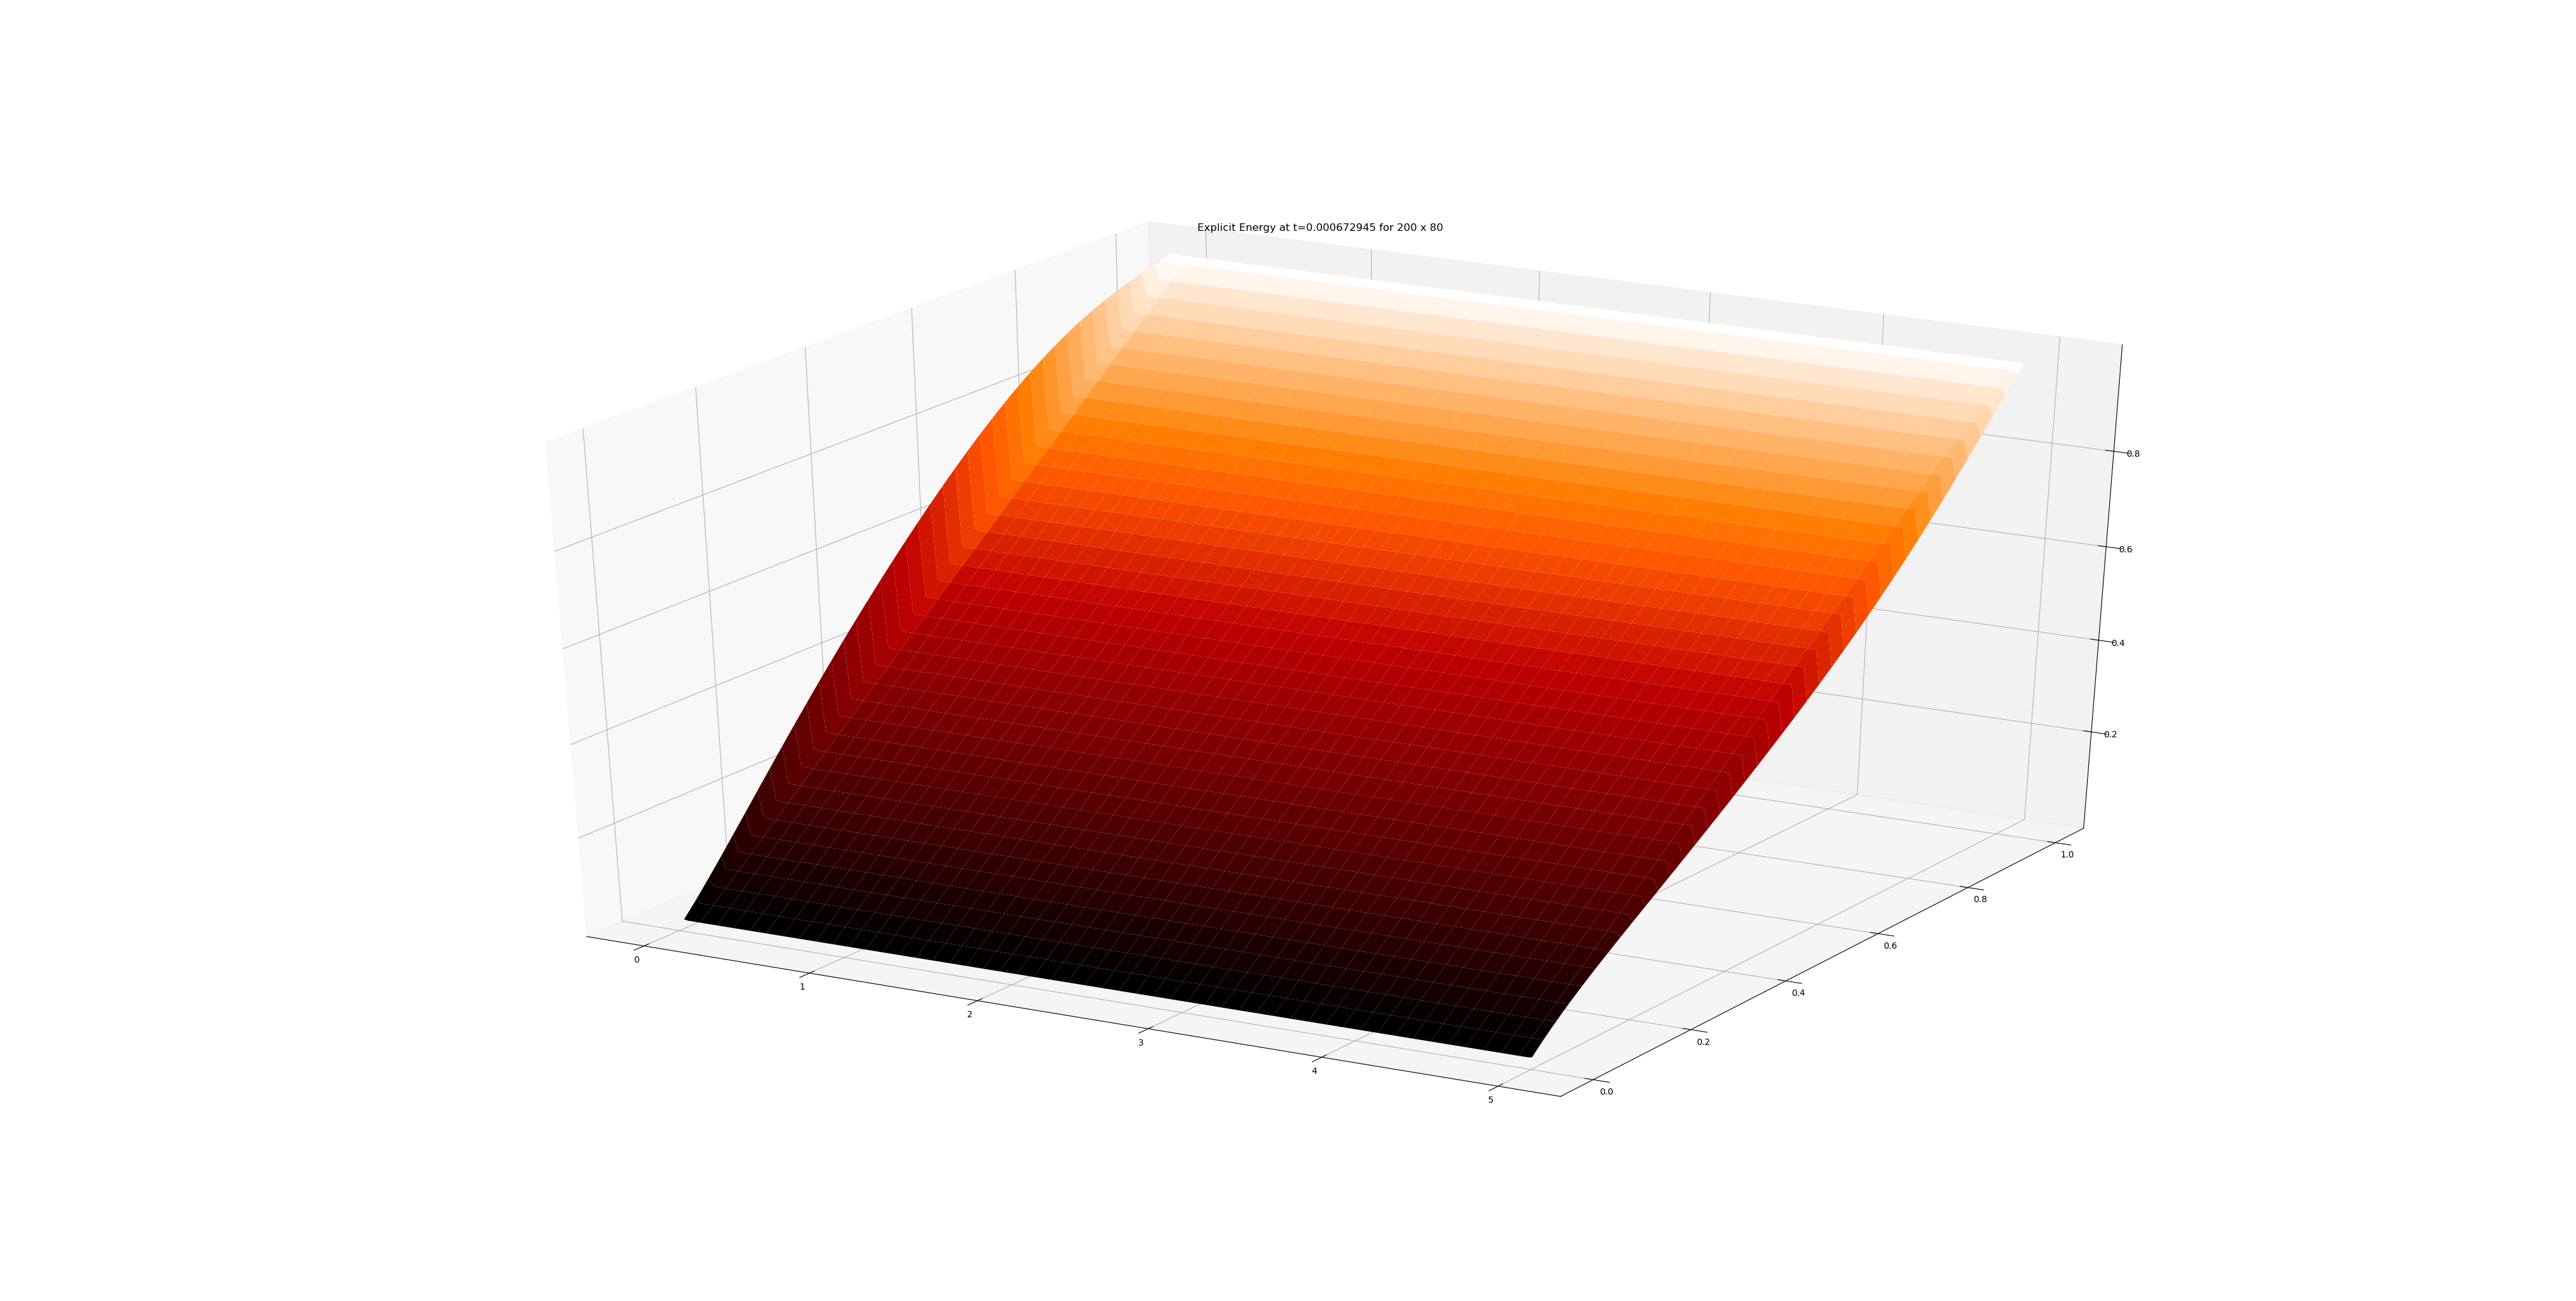
\includegraphics[width=0.6\textwidth]{figs/explicit_p5_0_0.png}
    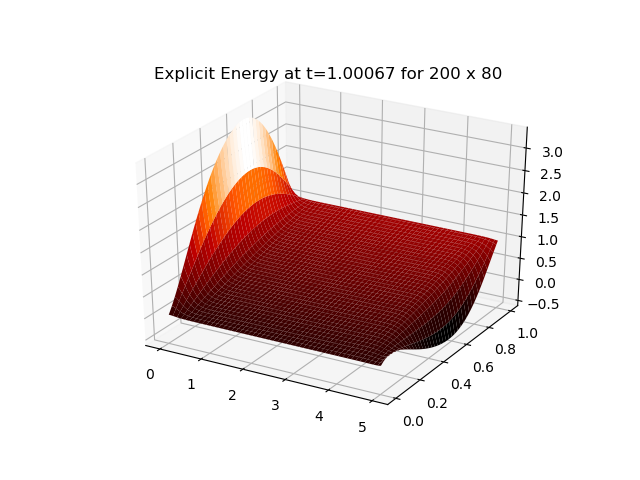
\includegraphics[width=0.6\textwidth]{figs/explicit_p5_1_0.png}
    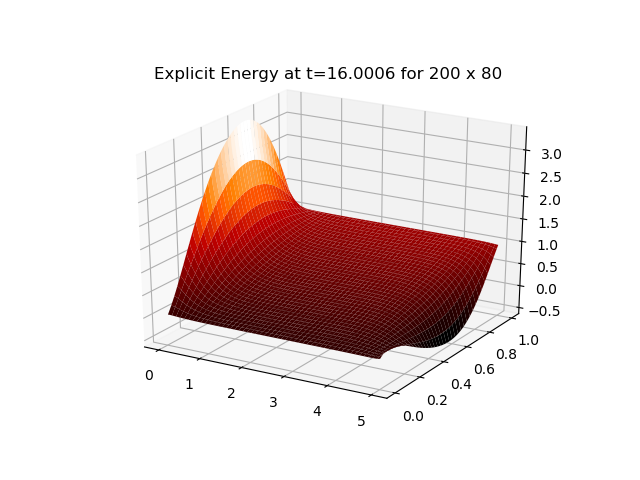
\includegraphics[width=0.6\textwidth]{figs/explicit_p5_16_0.png}
  }
  \caption{Temperature field from the explicit solver for the boundaries in problem 5 at times $t = 0, 1, 16$}
  \label{exp_part5}
\end{figure}

\begin{figure}[ht]
  \centering{
    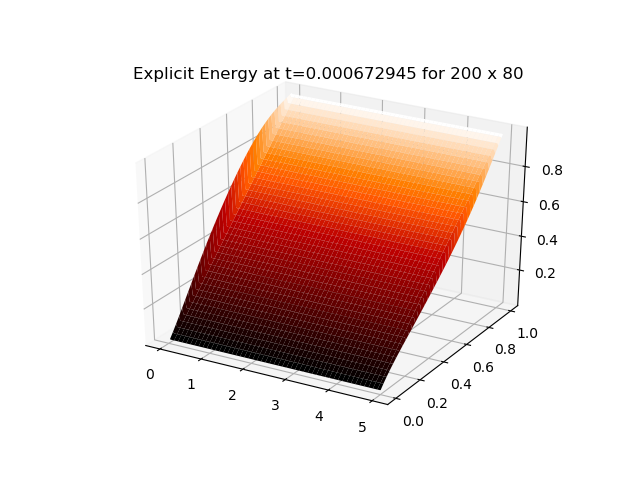
\includegraphics[width=0.6\textwidth]{figs/explicit_p7_0_0.png}
    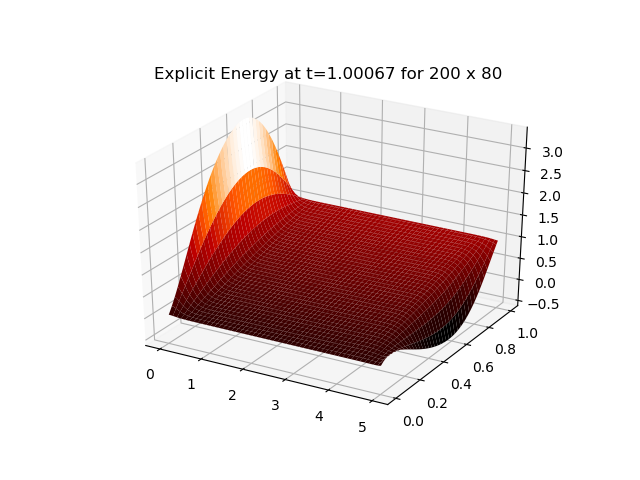
\includegraphics[width=0.6\textwidth]{figs/explicit_p7_1_0.png}
    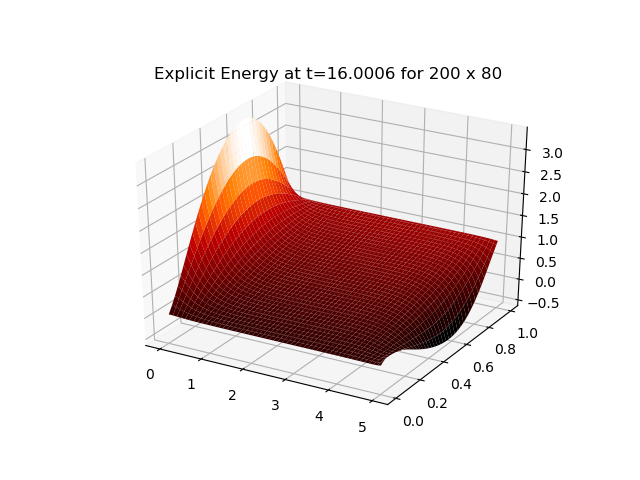
\includegraphics[width=0.6\textwidth]{figs/explicit_p7_16_0.png}
  }
  \caption{Temperature field from the explicit solver for the boundaries in problem 7 at times $t = 0, 1, 16$}
  \label{exp_part7}
\end{figure}

I do have performance measurements for my implicit solver, however.
While they do not reflect what the correct implementation would be,
they should be approximately correct,
since the correct implementation shouldn't be substantially different.
I list the amount of time for it takes for each solver to compute out
to $t = 1 s$ with a timestep that's about $80\%$ of the maximum stable step in Table \ref{timing}.

\begin{table}[ht]
  \centering{
    \begin{tabular}{|c|c|c|c|}
      \hline
      Solver & Mesh Size & Timestep & Time (ms)\\
      \hline
      RK 1 & $25 \times 10$  & 0.2800   & 0.01628\\
           & $50 \times 20$  & 0.07000  & 0.2641\\
           & $75 \times 30$  & 0.03111  & 1.334\\
           & $100 \times 40$ & 0.01750  & 3.463\\
           & $150 \times 60$ & 0.007778 & 17.83\\
           & $200 \times 80$ & 0.004375 & 54.01\\
      \hline
      RK 4 & $25 \times 10$  & 0.04307   & 0.4022\\
           & $50 \times 20$  & 0.01077   & 5.675\\
           & $75 \times 30$  & 0.004785  & 28.65\\
           & $100 \times 40$ & 0.002692  & 88.99\\
           & $150 \times 60$ & 0.001196  & 439.2\\
           & $200 \times 80$ & 0.0006729 & 138.4\\
      \hline
      Implicit & $25 \times 10$  & 0.1 & 0.1100\\
      Euler    & $50 \times 20$  & 0.1 & 0.3907\\
               & $75 \times 30$  & 0.1 & 0.8731\\
               & $100 \times 40$ & 0.1 & 1.541\\
               & $150 \times 60$ & 0.1 & 3.492\\
               & $200 \times 80$ & 0.1 & 6.822\\
      \hline
    \end{tabular}
  }
  \caption{Compute time required to reach $t=1.0$}
  \label{timing}
\end{table}

As expected, the timestep restriction causes the explicit solver to become extremely expensive as the mesh is refined,
while the implicit methods required time only increases linearly with the mesh size.

For the next project, I should reuse more of my previous code and focus on implementing features even when there are issues with the prior stages,
in addition to using a time dilation machine for more time.
\end{section}

\end{document}
